
\documentclass[a4paper, 12pt]{article}
\usepackage[left=3cm,right=1.5cm,top=2cm,bottom=2cm]{geometry}
\usepackage[T2A]{fontenc}
\usepackage{graphicx}

%Hyphenation rules
%--------------------------------------
\usepackage{hyphenat}
\hyphenation{ма-те-ма-ти-ка вос-ста-нав-ли-вать}
%--------------------------------------
\usepackage[english, russian]{babel}
\begin{document}
 
\tableofcontents

\begin{abstract}
  Это вводный абзац в начале документа.
\end{abstract}
 
\section{Задание}
\begin{enumerate}
\item Составить таблицу кодов блоков для метода Хаффмана с блокированием. Вероятности букв считать по фрагменту сообщения в задании. Длина блока указана. Вычислить EX, ML(X), ML(Xбл). Здесь EX – энтропия алфавита из букв сообщения, ML(X) – среднее количество элементарных символов на букву при сжатии методом Хаффмана, ML(Xбл) – среднее количество элементарных символов на букву при сжатии методом Хаффмана с блокированием. 
\item Сжать сообщение адаптивным методом Хаффмана. 
\item Сжать сообщение методами LZ77, LZSS, LZ78  Для методов LZ77, LZSS размер словаря – 10 символов, буфера – 6 символов. Для метода LZ78 размер словаря 32 записи. 
\item Сжать сообщение из задания №2 арифметическим методом. 
\item Распаковать сообщения, сжатые адаптивным методом Хаффмана, методами LZ77, LZSS, LZ78 и арифметическим методом. Для методов LZ77, LZSS размер словаря – 10 символов. Для метода LZ78 размер словаря – 16 записей. При декодировании таблица состоит из следующих столбцов: «Код», «Словарь» и «Выходной поток».
\end{enumerate}
\pagebreak
\section{Решение}
\subsection{Вариант №9}
\paragraph{Задание 1}

Строка СОКККККООО, размер блока: 2
\begin{center}
 \begin{tabular}{ |c|c|l| } 
  \hline
     Буква & Вероятность & Код\\ \hline
К & 0.50 & 0\\\hline
О & 0.40 & 11\\\hline
С & 0.10 & 10
\\ \hline \end{tabular}
\end{center}
Энтропия алфавита: 1.36
\begin{center}
 \begin{tabular}{ |c|c|l| } 
  \hline
     Блок & Вероятность & Код\\ \hline
КК & 0.25 & 10\\\hline
КО & 0.20 & 00\\\hline
ОК & 0.20 & 01\\\hline
ОО & 0.16 & 110\\\hline
КС & 0.05 & 11101\\\hline
СК & 0.05 & 11110\\\hline
ОС & 0.04 & 111111\\\hline
СО & 0.04 & 11100\\\hline
СС & 0.01 & 111110
\\ \hline \end{tabular}
\end{center}
Бит на символ при посимвольном кодировании: 1.50, при блочном: 1.39

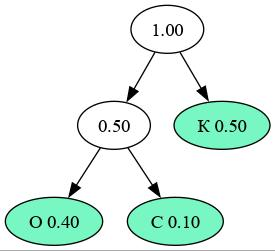
\includegraphics[width=0.5\linewidth]{/home/fizlrock/data/files/backup/code_backup/hobby/algoritms/LabExecutor/app/./doc_src/images/-1945050250.jpg}

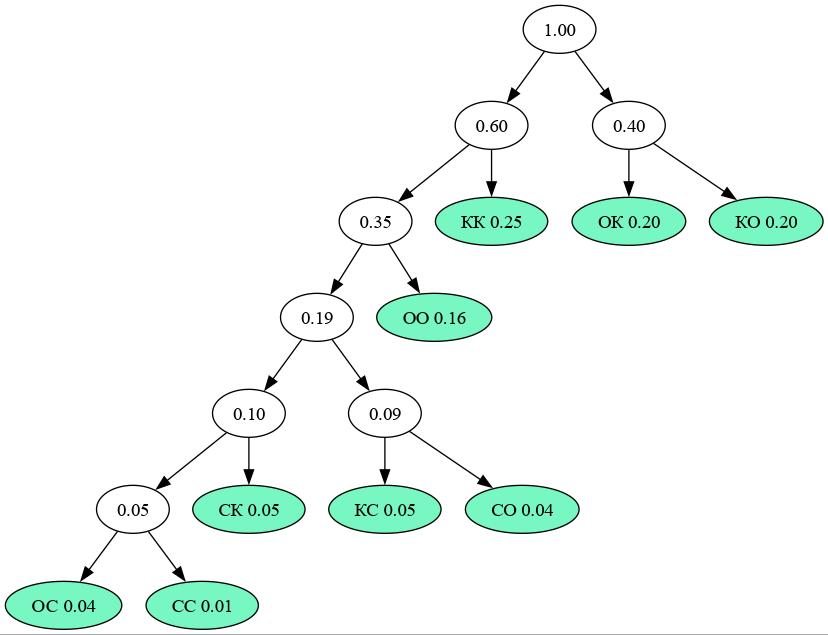
\includegraphics[width=0.9\linewidth]{/home/fizlrock/data/files/backup/code_backup/hobby/algoritms/LabExecutor/app/./doc_src/images/1265374033.jpg}
\end{document}